\section{Mathematik}
\subsection{Vektoren}

Darstellung:
	$\overrightarrow{a} = \mathbf{a} = \begin{bmatrix} a_1, a_2, a_3 \end{bmatrix} = \begin{bmatrix} a_1 \\ a_2 \\ a_3 \end{bmatrix}$


\begin{sectionbox}
	
	O bezeichnet den Ursprung (origo)
	
	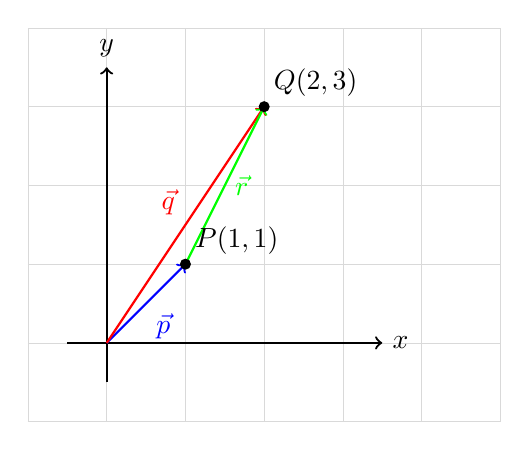
\begin{tikzpicture}
		% Draw grid
		\draw[help lines, color=gray!30] (-1,-1) grid (5,4);
		
		% Draw axes
		\draw[thick,->] (-0.5,0) -- (3.5,0) node[right] {$x$};
		\draw[thick,->] (0,-0.5) -- (0,3.5) node[above] {$y$};
		
		% Define points
		\coordinate (P) at (1,1);
		\coordinate (Q) at (2,3);
		
		% Draw vectors
		\draw[thick,->,blue] (0,0) -- (P) node[midway,below right] {$\vec{p}$};
		\draw[thick,->,red] (0,0) -- (Q) node[midway,above left] {$\vec{q}$};
		\draw[thick,->,green] (P) -- (Q) node[midway,right] {$\vec{r}$};
		% Draw and label points
		\fill (P) circle (2pt) node[above right] {$P (1,1)$};
		\fill (Q) circle (2pt) node[above right] {$Q (2,3)$};
		
	\end{tikzpicture}
	
	\begin{emphbox}
		$\overrightarrow{p} = \overrightarrow{OP} = \overrightarrow{P}$\\
		$\overrightarrow{q} = \overrightarrow{OQ} = \overrightarrow{Q}$\\
		$\overrightarrow{r} = \overrightarrow{PQ} = \overrightarrow{OQ} - \overrightarrow{OP} = \overrightarrow{q} - \overrightarrow{p}$\\
	\end{emphbox}



	Vektoraddition/-subtraktion
	\begin{emphbox}
		\begin{align*}
			\overrightarrow{a\pm b} = \overrightarrow{a} \pm \overrightarrow{b} = \begin{bmatrix} a_1 \pm b_1 \\ a_2 \pm b_2 \\ a_3 \pm b_3 \end{bmatrix}
		\end{align*}
	\end{emphbox}

	Assoziativ-/Distributivgesetz
	\begin{emphbox}
		\begin{align*}
			c_1 \cdot c_2 \cdot \overrightarrow{ab} = \overrightarrow{a}
		\end{align*}
	\end{emphbox}


	Normierter Vektor
	\begin{emphbox}
		\begin{align*}
			\overrightarrow{a_0} = \frac{\overrightarrow{a}}{|\overrightarrow{a}|} \text{Vektor mit Richtung von a, mit Länge 1}
		\end{align*}
	\end{emphbox}

	Multiplikation mit Skalar
	\begin{emphbox}
		\begin{align*}
			c \cdot \overrightarrow{a} = \begin{bmatrix} c \cdot a_1 \\ c \cdot a_2 \\ c \cdot a_3 \end{bmatrix}
		%	\left\{\right
		\end{align*}
	\end{emphbox}

	Skalarprodukt
	\begin{emphbox}
		\begin{align*}
			\overrightarrow{a} \cdot \overrightarrow{b} &= |\overrightarrow{a}| \cdot |\overrightarrow{b}| \cdot \cos \alpha \\
			\overrightarrow{a} \cdot \overrightarrow{b} &= \begin{bmatrix} a_1 \\ a_2 \\ a_3 \end{bmatrix} \cdot \begin{bmatrix} b_1 \\ b_2 \\ b_3 \end{bmatrix} = a_1 \cdot b_1 + a_2 \cdot b_2 + a_3 \cdot b_3 \\
			\overrightarrow{a} \perp \overrightarrow{b} &\Leftrightarrow \overrightarrow{a} \cdot \overrightarrow{b} = 0 
		\end{align*}
	\end{emphbox}

	Kreuzprodukt (Vektorprodukt)
	\begin{emphbox}
		$\overrightarrow{a} \times \overrightarrow{b} = \begin{bmatrix} a_1 \\ a_2 \\ a_3 \end{bmatrix} \times \begin{bmatrix} b_1 \\ b_2 \\ b_3 \end{bmatrix} = \begin{bmatrix} a_2 \cdot b_3 - a_3 \cdot b_2 \\ a_3 \cdot b_1 - a_1 \cdot b_3 \\ a_1 \cdot b_2 - a_2 \cdot b_1 \end{bmatrix} $
	\end{emphbox}
	
\end{sectionbox}
